% Curva de inversión f(I) = 4 sqrt(I), riqueza inicial D = 6, r = 25 %.
% Tangencia: f'(I) = 1 + r  =>  I = 2,56, J = 3,44, G = 6,4; K = J + G/1,25 = 8,56; M = G + 1,25 J = 10,7; H = 1,25 D = 7,5.
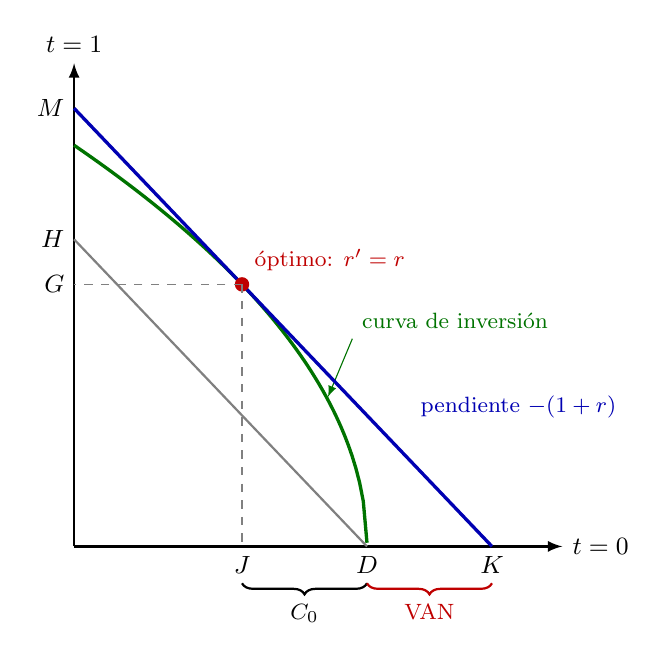
\begin{tikzpicture}[x=0.62cm, y=0.52cm, >=latex, font=\small]
  \draw[->, thick] (0,0) -- (10,0) node[right] {$t=0$};
  \draw[->, thick] (0,0) -- (0,11.8) node[above] {$t=1$};
  % Curva de oportunidades de inversión (cóncava)
  \draw[very thick, green!45!black, domain=0:6, samples=80] plot (\x,{4*sqrt(6-\x)});
  \node[green!45!black, anchor=west, font=\footnotesize] (ci) at (5.7,5.5) {curva de inversión};
  \draw[->, green!45!black] (ci.south west) -- (5.2,3.65);
  % Línea del mercado sin inversión real (D-H)
  \draw[thick, gray] (6,0) -- (0,7.5);
  % Línea del mercado tras invertir JD (K-M), tangente en (J,G)
  \draw[very thick, blue!70!black] (8.56,0) -- (0,10.7);
  % Punto de tangencia y proyecciones
  \fill[red!75!black] (3.44,6.4) circle (2.6pt);
  \draw[dashed, gray] (3.44,6.4) -- (3.44,0);
  \draw[dashed, gray] (3.44,6.4) -- (0,6.4);
  \node[anchor=south west, red!75!black, font=\footnotesize] at (3.5,6.5) {óptimo: $r' = r$};
  % Rótulos de los ejes
  \foreach \p/\l in {3.44/J, 6/D, 8.56/K} \node[below] at (\p,0) {$\l$};
  \foreach \p/\l in {6.4/G, 7.5/H, 10.7/M} \node[left] at (0,\p) {$\l$};
  % Segmentos JD (inversión), DK (VAN)
  \draw[decorate, decoration={brace, mirror, amplitude=4pt}, thick] (3.44,-0.9) -- (6,-0.9)
     node[midway, below=4pt, font=\footnotesize] {$C_0$};
  \draw[decorate, decoration={brace, mirror, amplitude=4pt}, thick, red!75!black] (6,-0.9) -- (8.56,-0.9)
     node[midway, below=4pt, font=\footnotesize] {VAN};
  \node[blue!70!black, font=\footnotesize, anchor=west] at (6.9,3.4) {pendiente $-(1+r)$};
\end{tikzpicture}
